% Options for packages loaded elsewhere
\PassOptionsToPackage{unicode}{hyperref}
\PassOptionsToPackage{hyphens}{url}
%
\documentclass[
  english,
  man,floatsintext]{apa6}
\usepackage{lmodern}
\usepackage{amssymb,amsmath}
\usepackage{ifxetex,ifluatex}
\ifnum 0\ifxetex 1\fi\ifluatex 1\fi=0 % if pdftex
  \usepackage[T1]{fontenc}
  \usepackage[utf8]{inputenc}
  \usepackage{textcomp} % provide euro and other symbols
\else % if luatex or xetex
  \usepackage{unicode-math}
  \defaultfontfeatures{Scale=MatchLowercase}
  \defaultfontfeatures[\rmfamily]{Ligatures=TeX,Scale=1}
\fi
% Use upquote if available, for straight quotes in verbatim environments
\IfFileExists{upquote.sty}{\usepackage{upquote}}{}
\IfFileExists{microtype.sty}{% use microtype if available
  \usepackage[]{microtype}
  \UseMicrotypeSet[protrusion]{basicmath} % disable protrusion for tt fonts
}{}
\makeatletter
\@ifundefined{KOMAClassName}{% if non-KOMA class
  \IfFileExists{parskip.sty}{%
    \usepackage{parskip}
  }{% else
    \setlength{\parindent}{0pt}
    \setlength{\parskip}{6pt plus 2pt minus 1pt}}
}{% if KOMA class
  \KOMAoptions{parskip=half}}
\makeatother
\usepackage{xcolor}
\IfFileExists{xurl.sty}{\usepackage{xurl}}{} % add URL line breaks if available
\IfFileExists{bookmark.sty}{\usepackage{bookmark}}{\usepackage{hyperref}}
\hypersetup{
  pdftitle={grafzahl: fine-tuning Transformers for text data from within R},
  pdfauthor={Chung-hong Chan1},
  pdflang={en-EN},
  pdfkeywords={machine learning, transformers, R, python, automated content analysis},
  hidelinks,
  pdfcreator={LaTeX via pandoc}}
\urlstyle{same} % disable monospaced font for URLs
\usepackage{color}
\usepackage{fancyvrb}
\newcommand{\VerbBar}{|}
\newcommand{\VERB}{\Verb[commandchars=\\\{\}]}
\DefineVerbatimEnvironment{Highlighting}{Verbatim}{commandchars=\\\{\}}
% Add ',fontsize=\small' for more characters per line
\usepackage{framed}
\definecolor{shadecolor}{RGB}{248,248,248}
\newenvironment{Shaded}{\begin{snugshade}}{\end{snugshade}}
\newcommand{\AlertTok}[1]{\textcolor[rgb]{0.94,0.16,0.16}{#1}}
\newcommand{\AnnotationTok}[1]{\textcolor[rgb]{0.56,0.35,0.01}{\textbf{\textit{#1}}}}
\newcommand{\AttributeTok}[1]{\textcolor[rgb]{0.77,0.63,0.00}{#1}}
\newcommand{\BaseNTok}[1]{\textcolor[rgb]{0.00,0.00,0.81}{#1}}
\newcommand{\BuiltInTok}[1]{#1}
\newcommand{\CharTok}[1]{\textcolor[rgb]{0.31,0.60,0.02}{#1}}
\newcommand{\CommentTok}[1]{\textcolor[rgb]{0.56,0.35,0.01}{\textit{#1}}}
\newcommand{\CommentVarTok}[1]{\textcolor[rgb]{0.56,0.35,0.01}{\textbf{\textit{#1}}}}
\newcommand{\ConstantTok}[1]{\textcolor[rgb]{0.00,0.00,0.00}{#1}}
\newcommand{\ControlFlowTok}[1]{\textcolor[rgb]{0.13,0.29,0.53}{\textbf{#1}}}
\newcommand{\DataTypeTok}[1]{\textcolor[rgb]{0.13,0.29,0.53}{#1}}
\newcommand{\DecValTok}[1]{\textcolor[rgb]{0.00,0.00,0.81}{#1}}
\newcommand{\DocumentationTok}[1]{\textcolor[rgb]{0.56,0.35,0.01}{\textbf{\textit{#1}}}}
\newcommand{\ErrorTok}[1]{\textcolor[rgb]{0.64,0.00,0.00}{\textbf{#1}}}
\newcommand{\ExtensionTok}[1]{#1}
\newcommand{\FloatTok}[1]{\textcolor[rgb]{0.00,0.00,0.81}{#1}}
\newcommand{\FunctionTok}[1]{\textcolor[rgb]{0.00,0.00,0.00}{#1}}
\newcommand{\ImportTok}[1]{#1}
\newcommand{\InformationTok}[1]{\textcolor[rgb]{0.56,0.35,0.01}{\textbf{\textit{#1}}}}
\newcommand{\KeywordTok}[1]{\textcolor[rgb]{0.13,0.29,0.53}{\textbf{#1}}}
\newcommand{\NormalTok}[1]{#1}
\newcommand{\OperatorTok}[1]{\textcolor[rgb]{0.81,0.36,0.00}{\textbf{#1}}}
\newcommand{\OtherTok}[1]{\textcolor[rgb]{0.56,0.35,0.01}{#1}}
\newcommand{\PreprocessorTok}[1]{\textcolor[rgb]{0.56,0.35,0.01}{\textit{#1}}}
\newcommand{\RegionMarkerTok}[1]{#1}
\newcommand{\SpecialCharTok}[1]{\textcolor[rgb]{0.00,0.00,0.00}{#1}}
\newcommand{\SpecialStringTok}[1]{\textcolor[rgb]{0.31,0.60,0.02}{#1}}
\newcommand{\StringTok}[1]{\textcolor[rgb]{0.31,0.60,0.02}{#1}}
\newcommand{\VariableTok}[1]{\textcolor[rgb]{0.00,0.00,0.00}{#1}}
\newcommand{\VerbatimStringTok}[1]{\textcolor[rgb]{0.31,0.60,0.02}{#1}}
\newcommand{\WarningTok}[1]{\textcolor[rgb]{0.56,0.35,0.01}{\textbf{\textit{#1}}}}
\usepackage{graphicx}
\makeatletter
\def\maxwidth{\ifdim\Gin@nat@width>\linewidth\linewidth\else\Gin@nat@width\fi}
\def\maxheight{\ifdim\Gin@nat@height>\textheight\textheight\else\Gin@nat@height\fi}
\makeatother
% Scale images if necessary, so that they will not overflow the page
% margins by default, and it is still possible to overwrite the defaults
% using explicit options in \includegraphics[width, height, ...]{}
\setkeys{Gin}{width=\maxwidth,height=\maxheight,keepaspectratio}
% Set default figure placement to htbp
\makeatletter
\def\fps@figure{htbp}
\makeatother
\setlength{\emergencystretch}{3em} % prevent overfull lines
\providecommand{\tightlist}{%
  \setlength{\itemsep}{0pt}\setlength{\parskip}{0pt}}
\setcounter{secnumdepth}{-\maxdimen} % remove section numbering
% Make \paragraph and \subparagraph free-standing
\ifx\paragraph\undefined\else
  \let\oldparagraph\paragraph
  \renewcommand{\paragraph}[1]{\oldparagraph{#1}\mbox{}}
\fi
\ifx\subparagraph\undefined\else
  \let\oldsubparagraph\subparagraph
  \renewcommand{\subparagraph}[1]{\oldsubparagraph{#1}\mbox{}}
\fi
% Manuscript styling
\usepackage{upgreek}
\captionsetup{font=singlespacing,justification=justified}

% Table formatting
\usepackage{longtable}
\usepackage{lscape}
% \usepackage[counterclockwise]{rotating}   % Landscape page setup for large tables
\usepackage{multirow}		% Table styling
\usepackage{tabularx}		% Control Column width
\usepackage[flushleft]{threeparttable}	% Allows for three part tables with a specified notes section
\usepackage{threeparttablex}            % Lets threeparttable work with longtable

% Create new environments so endfloat can handle them
% \newenvironment{ltable}
%   {\begin{landscape}\centering\begin{threeparttable}}
%   {\end{threeparttable}\end{landscape}}
\newenvironment{lltable}{\begin{landscape}\centering\begin{ThreePartTable}}{\end{ThreePartTable}\end{landscape}}

% Enables adjusting longtable caption width to table width
% Solution found at http://golatex.de/longtable-mit-caption-so-breit-wie-die-tabelle-t15767.html
\makeatletter
\newcommand\LastLTentrywidth{1em}
\newlength\longtablewidth
\setlength{\longtablewidth}{1in}
\newcommand{\getlongtablewidth}{\begingroup \ifcsname LT@\roman{LT@tables}\endcsname \global\longtablewidth=0pt \renewcommand{\LT@entry}[2]{\global\advance\longtablewidth by ##2\relax\gdef\LastLTentrywidth{##2}}\@nameuse{LT@\roman{LT@tables}} \fi \endgroup}

% \setlength{\parindent}{0.5in}
% \setlength{\parskip}{0pt plus 0pt minus 0pt}

% Overwrite redefinition of paragraph and subparagraph by the default LaTeX template
% See https://github.com/crsh/papaja/issues/292
\makeatletter
\renewcommand{\paragraph}{\@startsection{paragraph}{4}{\parindent}%
  {0\baselineskip \@plus 0.2ex \@minus 0.2ex}%
  {-1em}%
  {\normalfont\normalsize\bfseries\itshape\typesectitle}}

\renewcommand{\subparagraph}[1]{\@startsection{subparagraph}{5}{1em}%
  {0\baselineskip \@plus 0.2ex \@minus 0.2ex}%
  {-\z@\relax}%
  {\normalfont\normalsize\itshape\hspace{\parindent}{#1}\textit{\addperi}}{\relax}}
\makeatother

% \usepackage{etoolbox}
\makeatletter
\patchcmd{\HyOrg@maketitle}
  {\section{\normalfont\normalsize\abstractname}}
  {\section*{\normalfont\normalsize\abstractname}}
  {}{\typeout{Failed to patch abstract.}}
\patchcmd{\HyOrg@maketitle}
  {\section{\protect\normalfont{\@title}}}
  {\section*{\protect\normalfont{\@title}}}
  {}{\typeout{Failed to patch title.}}
\makeatother

\usepackage{xpatch}
\makeatletter
\xapptocmd\appendix
  {\xapptocmd\section
    {\addcontentsline{toc}{section}{\appendixname\ifoneappendix\else~\theappendix\fi\\: #1}}
    {}{\InnerPatchFailed}%
  }
{}{\PatchFailed}
\keywords{machine learning, transformers, R, python, automated content analysis\newline\indent Word count: 2018}
\usepackage{csquotes}
\ifxetex
  % Load polyglossia as late as possible: uses bidi with RTL langages (e.g. Hebrew, Arabic)
  \usepackage{polyglossia}
  \setmainlanguage[]{english}
\else
  \usepackage[shorthands=off,main=english]{babel}
\fi
\newlength{\cslhangindent}
\setlength{\cslhangindent}{1.5em}
\newenvironment{cslreferences}%
  {\setlength{\parindent}{0pt}%
  \everypar{\setlength{\hangindent}{\cslhangindent}}\ignorespaces}%
  {\par}

\title{grafzahl: fine-tuning Transformers for text data from within R}
\author{Chung-hong Chan\textsuperscript{1}}
\date{}


\shorttitle{PUT THE R BACK IN TRANSFORMERS}

\authornote{

Source code and data are available at \url{https://github.com/chainsawriot/grafzahl}. I would like to thank 1) Jarvis Labs for providing discounted GPU cloud service for the development of this package; 2) Pablo Barberá (University of Southern California) and Wouter van Atteveldt (VU Amsterdam) for allowing me to include their datasets in this package.

Correspondence concerning this article should be addressed to Chung-hong Chan, Unter Sachsenhausen 6-8, 50667 Köln. E-mail: \href{mailto:chung-hong.chan@gesis.org}{\nolinkurl{chung-hong.chan@gesis.org}}

}

\affiliation{\vspace{0.5cm}\textsuperscript{1} GESIS - Leibniz-Institut für Sozialwissenschaften, Germany}

\abstract{%
This paper introduces \texttt{grafzahl}, an R package for fine-tuning Transformers for text data from within R. The package is used in this paper to reproduce the analyses in communication papers or, of non-Germanic benchmark datasets. Very significant improvement in model accuacy over traditional machine learning approach such as Convoluted Neural Network is observed.
}



\begin{document}
\maketitle

\hypertarget{put-the-r-back-in-transformers}{%
\subsection{Put the R back in Transformers}\label{put-the-r-back-in-transformers}}

The purpose of this R package, \texttt{grafzahl}, is to provide the missing link between R and modern Transformers language models. Under the hood, the training part is based on the Python packages \texttt{transformers} (Wolf et al., 2020) and \texttt{simpletransformers} (Rajapakse, 2022). The integration based on \texttt{reticulate} (Ushey, Allaire, \& Tang, 2022) is seamless. With this seamless integration provided, communication researchers can produce the most advanced supervised learning models entirely from within R. This package provides the function \texttt{grafzahl()}, which emulates the behaviors of \texttt{quanteda.textmodels} (Benoit et al., 2021).\footnote{This package uses reasonable default settings which suit what communication researchers would like to achieve with these models. But the package also provides the freedom for communication researchers to finely adjust the parameters for their specific applications. However, the reanalysis of several examples in communication suggests that even the default settings can generate great improvement over the performance as reported in the original papers. Also, there is almost no need to conduct the cumbersome proprocessing and feature engineering steps, which all examples originally required.}

Two examples (Azime \& Mohammed, 2021; Van Atteveldt, Van der Velden, \& Boukes, 2021) are presented here. Additional examples (Çöltekin, 2020; Dobbrick, Jakob, Chan, \& Wessler, 2021; Theocharis, Barberá, Fazekas, \& Popa, 2020) are available in the Github repository of the package (\url{https://github.com/chainsawriot/grafzahl}).

\hypertarget{monolingual-classification-example}{%
\section{Monolingual classification example}\label{monolingual-classification-example}}

Van Atteveldt et al. (2021) compare various methods to analyze the tone of Dutch economic news' headlines. Headlines were coded into three categories: negative (-1), neutral (0), and positive (+1).

In the original paper, Van Atteveldt et al. (2021) show that the best method for predicting expert coding, other than coding by student helpers, is convoluted neural network (CNN) with Dutch word embeddings trained on Dutch news. The out-of-sample F1 of .63, .66, and .56 were reported for the three categories. As the data (including the training-and-test split) are publicly available\footnote{\url{https://github.com/vanatteveldt/ecosent/}} and included in this package (as \texttt{ecosent}), I can provide a head-to-head comparison between the reported CNN and the Transformer-based model trained with \texttt{grafzahl}.

There are three important columns in the \texttt{ecosent} data frame:

\begin{enumerate}
\def\labelenumi{\arabic{enumi}.}
\tightlist
\item
  \texttt{headline}: the actual text data
\item
  \texttt{value}: the sentiment
\item
  \texttt{gold}: whether or not this row is ``gold standard'', i.e.~test set. There are 6,038 and 300 headlines in the training and test set respectively.
\end{enumerate}

\hypertarget{workflow}{%
\subsection{Workflow}\label{workflow}}

\hypertarget{step-0-setup-grafzahl}{%
\subsubsection{\texorpdfstring{Step 0: Setup \texttt{grafzahl}}{Step 0: Setup grafzahl}}\label{step-0-setup-grafzahl}}

This step only needs to be done once. A miniconda environment needs to be setup. It is in general not recommended to use this package without a CUDA-compatible GPU. Without a CUDA-compatible GPU, the fine-tuning processes below might take days, if not weeks.

If there is a GPU capable of performing CUDA, run:

\begin{Shaded}
\begin{Highlighting}[]
\KeywordTok{require}\NormalTok{(grafzahl)}
\KeywordTok{setup\_grafzahl}\NormalTok{(}\DataTypeTok{cuda =} \OtherTok{TRUE}\NormalTok{) }\CommentTok{\# set to FALSE otherwise}
\KeywordTok{detect\_cuda}\NormalTok{()}
\end{Highlighting}
\end{Shaded}

If the automatic setup failed, one can also set up the miniconda environment manually to diagnose what went wrong. The complete instructions are available here: \url{https://github.com/chainsawriot/grafzahl/wiki/setup_grafzahl}

\hypertarget{step-1-get-information-of-the-pretrained-transformer}{%
\subsubsection{Step 1: Get information of the pretrained Transformer}\label{step-1-get-information-of-the-pretrained-transformer}}

The first step of training a Transformer-based model is to find a suitable pretrained Transformer model on Hugging Face,\footnote{Hugging Face (\url{https://huggingface.co}) is an online repository of pretrained machine learning models.} which would work for the data. As the data are in Dutch, the pretrained Dutch Transformer model BERTje should work (de Vries et al., 2019, available from \url{https://huggingface.co/GroNLP/bert-base-dutch-cased}). The model name of BERTje is \texttt{GroNLP/bert-base-dutch-cased}. It is also important to note the citation information to properly cite the pretrained Transformer model.

\hypertarget{step-2-create-the-corpus}{%
\subsubsection{Step 2: Create the corpus}\label{step-2-create-the-corpus}}

The second step is to read the data as a corpus.\footnote{This step is not absolutely needed. The package can also work with character vectors. The \texttt{corpus} data structure is a better representation of character vector.}

\begin{Shaded}
\begin{Highlighting}[]
\KeywordTok{require}\NormalTok{(readtext)}
\KeywordTok{require}\NormalTok{(quanteda)}
\NormalTok{input \textless{}{-}}\StringTok{ }\KeywordTok{corpus}\NormalTok{(ecosent, }\DataTypeTok{text\_field =} \StringTok{"headline"}\NormalTok{)}
\end{Highlighting}
\end{Shaded}

We can manipulate the corpus object using the functions provided by \texttt{quanteda}. For example, one can subset the training set using the function \texttt{corpus\_subset()}.

\begin{Shaded}
\begin{Highlighting}[]
\CommentTok{\#\# selecting documents where the docvar \textasciigrave{}gold\textasciigrave{} is FALSE}
\NormalTok{training\_corpus \textless{}{-}}\StringTok{ }\KeywordTok{corpus\_subset}\NormalTok{(input, }\OperatorTok{!}\NormalTok{gold)}
\end{Highlighting}
\end{Shaded}

\hypertarget{step-3-fine-tune-the-model}{%
\subsubsection{Step 3: Fine-tune the model}\label{step-3-fine-tune-the-model}}

With the corpus and model name, the \texttt{grafzahl} function is used to fine-tune the model.

\begin{Shaded}
\begin{Highlighting}[]
\NormalTok{model \textless{}{-}}\StringTok{ }\KeywordTok{grafzahl}\NormalTok{(}\DataTypeTok{x =}\NormalTok{ training\_corpus,}
                  \DataTypeTok{y =} \StringTok{"value"}\NormalTok{,}
                  \DataTypeTok{model\_name =} \StringTok{"GroNLP/bert{-}base{-}dutch{-}cased"}\NormalTok{)}
\end{Highlighting}
\end{Shaded}

In general, it is better to specify \texttt{output\_dir} (where to put the saved model object). By default, it will be \texttt{output} a random temporary directory. The R function \texttt{set.seed()} can also be used to preserve the random seed for reproducibility.

On a regular off-the-shelf gaming laptop with a GeForce RTX 3050 Ti GPU and 4G of GPU ram, the process took around 20 minutes.

\hypertarget{step-4-make-prediction}{%
\subsubsection{Step 4: Make prediction}\label{step-4-make-prediction}}

Following the convention of \texttt{lm()} and many other R packages, the object returned by the function \texttt{grafzahl()} has a \texttt{predict()} S3 method. The following code gets the predicted sentiment of the headlines in the test set.

\begin{Shaded}
\begin{Highlighting}[]
\NormalTok{test\_corpus \textless{}{-}}\StringTok{ }\KeywordTok{corpus\_subset}\NormalTok{(input, gold)}
\NormalTok{predicted\_sentiment \textless{}{-}}\StringTok{ }\KeywordTok{predict}\NormalTok{(model, test\_corpus)}
\end{Highlighting}
\end{Shaded}

\hypertarget{step-5-evaluate-performance}{%
\subsubsection{Step 5: Evaluate performance}\label{step-5-evaluate-performance}}

With the predicted sentiment and the ground truth, there are many ways to evaluate the performance of the fine-tuned model. The simplest way is to construct a confusion matrix using the standard \texttt{table()} function.

\begin{Shaded}
\begin{Highlighting}[]
\NormalTok{cm \textless{}{-}}\StringTok{ }\KeywordTok{table}\NormalTok{(predicted\_sentiment,}
            \DataTypeTok{ground\_truth =} \KeywordTok{docvars}\NormalTok{(test\_corpus, }\StringTok{"value"}\NormalTok{))}
\end{Highlighting}
\end{Shaded}

The R package \texttt{caret} (Kuhn, 2008) can also be used to calculate standard performance metrics such as Precision, Recall, and F1.\footnote{The function \texttt{confusionMatrix()} can accept the predicted values and ground truth directly, without using \texttt{table()} first. But the predicted values and ground truth must be \texttt{factor}: \texttt{confusionMatrix(as.factor(predicted\_sentiment),\ as.factor(docvars(test\_corpus,\ "value")),\ mode\ =\ "prec\_recall")}.}

\begin{Shaded}
\begin{Highlighting}[]
\KeywordTok{require}\NormalTok{(caret)}
\KeywordTok{confusionMatrix}\NormalTok{(cm, }\DataTypeTok{mode =} \StringTok{"prec\_recall"}\NormalTok{)}
\end{Highlighting}
\end{Shaded}

The out-of-sample F1 measures of the fine-tuned model are .76, .67, and .72 (vs reported .63, .66, and .56). There is great improvement over the CNN model reported by Van Atteveldt et al. (2021), although the prediction accuracy for the neutral category is just on par. Van Atteveldt et al. (2021) also provide the learning curve of CNN and Support Vector Machine (SVM). A learning curve plots the out-of-sample prediction performance as a function of number of training examples. I repeat the analysis in a similar manner to Van Atteveldt et al. (2021) and plot the learning curve of Transformer-based model trained using the default workflow of \texttt{grafzahl}.

Figure \ref{fig:fig2} show the fine-tuned Transformer model's learning curve alongside CNN's and SVM's.\footnote{The R code for generating the learning curves is available in the official repository: \url{https://github.com/chainsawriot/grafzahl}} The fune-tuned model has much better performance than CNN and SVM even with only 500 training examples. Unlike CNN and SVM, the gain in performance appears to plateau after 2500. It points to the fact that one does not need to have a lot of training data to fine-tune a Transformer model.

\begin{figure}
\centering
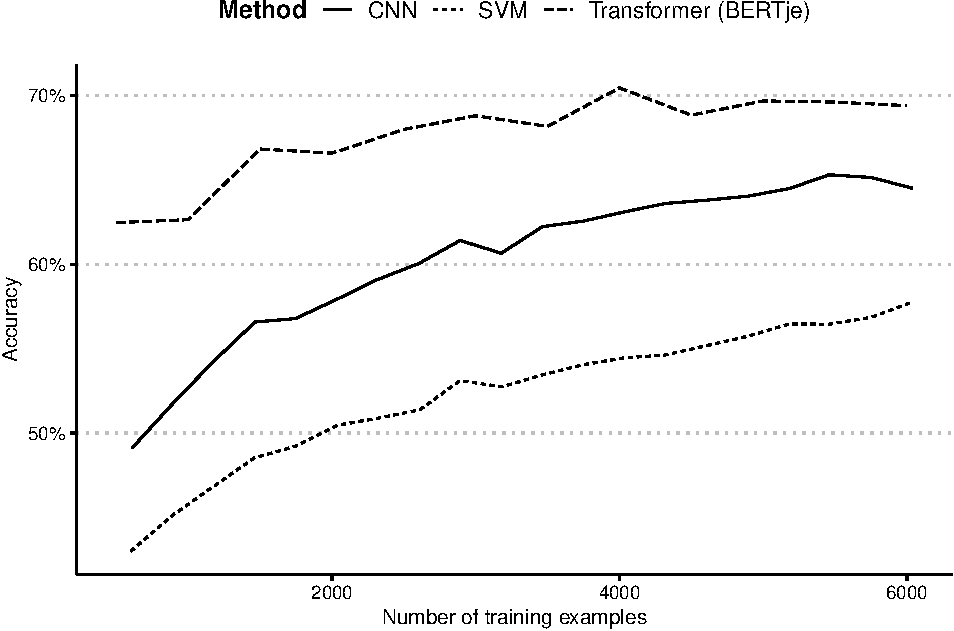
\includegraphics{grafzahl_sp_files/figure-latex/fig2-1.pdf}
\caption{\label{fig:fig2}Learning curve of machine learning algorithms}
\end{figure}

\hypertarget{step-5-explain-the-prediction}{%
\subsubsection{Step 5: Explain the prediction}\label{step-5-explain-the-prediction}}

Unlike ``glass-box'' machine learning models (Dobbrick et al., 2021), Transformer-based prediction models are ``black-box''. There are so many parameters in Transformers (the BERT base model has 110 million parameters) and this complexity makes each individual parameter of a model not interpretable.

A reasonable compromise is to make the prediction \emph{explainable} instead. Generating Local Interpretable Model-agnostic Explanations (LIME) (Ribeiro, Singh, \& Guestrin, 2016; R implementation by Pedersen \& Benesty, 2021) is a good way to explain how the model makes its prediction. The gist of the method is to perturb the input text data by deleting parts of the sentence. For example: the sentence ``I hate this movie'' will be perturbed as ``I this movie'', ``I hate movie'', ``I hate this'', ``I hate'' etc. These perturbed sentences are then feed into the machine learning model to make predictions. The relationship between what get deleted and the prediction is studied. The parts that change the prediction a lot would be more \emph{causal} to the original prediction.

With the trained model, we can explain the predictions made for the following two Dutch headlines: \emph{``Dijsselbloem pessimistisch over snelle stappen Grieken''} (Dijsselbloem {[}the Former Minister of Finance of the Netherlands{]} pessimistic about rapid maneuvers from Greeks) and \emph{``Aandelenbeurzen zetten koersopmars voort''} (Stock markets continue to rise). Models trained with \texttt{grafzahl} support the R package \texttt{lime} directly. One can get explanations using the following code:

\begin{Shaded}
\begin{Highlighting}[]
\KeywordTok{require}\NormalTok{(lime)}
\NormalTok{sentences \textless{}{-}}\StringTok{ }\KeywordTok{c}\NormalTok{(}\StringTok{"Dijsselbloem pessimistisch over snelle stappen Grieken"}\NormalTok{,}
               \StringTok{"Aandelenbeurzen zetten koersopmars voort"}\NormalTok{)}
\NormalTok{explainer \textless{}{-}}\StringTok{ }\KeywordTok{lime}\NormalTok{(training\_corpus, model)}
\NormalTok{explanations \textless{}{-}}\StringTok{ }\KeywordTok{explain}\NormalTok{(sentences, explainer, }\DataTypeTok{n\_labels =} \DecValTok{1}\NormalTok{,}
                        \DataTypeTok{n\_features =} \DecValTok{3}\NormalTok{)}
\KeywordTok{plot\_text\_explanations}\NormalTok{(explanations)}
\end{Highlighting}
\end{Shaded}

\begin{figure}
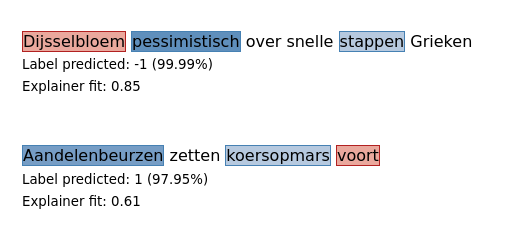
\includegraphics[width=1\linewidth]{fig1} \caption{Generating Local Interpretable Model-agnostic Explanations (LIME) of two predictions from the trained Dutch sentiment model}\label{fig:fig1}
\end{figure}

Figure \ref{fig:fig1} shows that for the sentence \emph{``Dijsselbloem pessimistisch over snelle stappen Grieken''} (classified as negative), the tokens \emph{pessimistisch} and \emph{stappen} are making the prediction towards the classified position (negative). But the token \emph{Dijsselbloem} is making it away.

\hypertarget{non-germanic-example-amharic}{%
\section{Non-Germanic example: Amharic}\label{non-germanic-example-amharic}}

I want to emphasize that \texttt{grafzahl} is not just another package focusing only on English, or Germanic languages such as Dutch. Baden, Pipal, Schoonvelde, and van der Velden (2021) criticize this tendency.

Amharic is a Semitic language mainly spoken in Ethiopia and is in general considered to be a ``low resource'' language. (Joshi, Santy, Budhiraja, Bali, \& Choudhury, 2020) Only recently, the first news classification dataset called ``Amharic News Text classification Dataset'' is available (Azime \& Mohammed, 2021). The dataset contains 50,706 news articles curated from various Amharic websites. The original paper reports the baseline out-of-sample accuracy of 62.2\% using Naive Bayes. The released data also contains the training-and-test split.\footnote{\url{https://huggingface.co/datasets/israel/Amharic-News-Text-classification-Dataset}} In this example, the AfriBERTa is used as the pretrained model (Ogueji, Zhu, \& Lin, 2021). The AfriBERTa model was trained with a small corpus of 11 African languages. Similar to the previous example, the default settings of \texttt{grafzahl} are used.

\begin{Shaded}
\begin{Highlighting}[]
\NormalTok{input \textless{}{-}}\StringTok{ }\KeywordTok{get\_amharic\_data}\NormalTok{()}
\NormalTok{model \textless{}{-}}\StringTok{ }\KeywordTok{grafzahl}\NormalTok{(}\DataTypeTok{x =}\NormalTok{ input}\OperatorTok{$}\NormalTok{training,}
                  \DataTypeTok{y =} \StringTok{"category"}\NormalTok{,}
                  \DataTypeTok{model\_name =} \StringTok{"castorini/afriberta\_base"}\NormalTok{)}

\CommentTok{\#\# Calculate the out{-}of{-}sample accuracy}

\NormalTok{preds \textless{}{-}}\StringTok{ }\KeywordTok{predict}\NormalTok{(model, }\DataTypeTok{newdata =}\NormalTok{ input}\OperatorTok{$}\NormalTok{test)}
\NormalTok{caret}\OperatorTok{::}\KeywordTok{confusionMatrix}\NormalTok{(}\KeywordTok{table}\NormalTok{(preds, }\KeywordTok{docvars}\NormalTok{(input}\OperatorTok{$}\NormalTok{test, }\StringTok{"category"}\NormalTok{)))}
\end{Highlighting}
\end{Shaded}

\hypertarget{results}{%
\subsection{Results}\label{results}}

The final out-of-sample accuracy is 84.18\%, a solid improvement from the baseline of 62.2\%.

\hypertarget{conclusion}{%
\section{Conclusion}\label{conclusion}}

This paper presents the R packages \texttt{grafzahl} and demonstrates its applicability to communication research by replicating the supervised machine learning part of published communication research.

\hypertarget{references}{%
\section{References}\label{references}}

\begingroup
\setlength{\parindent}{-0.5in}
\setlength{\leftskip}{0.5in}

\hypertarget{refs}{}
\begin{cslreferences}
\leavevmode\hypertarget{ref-azime2021amharic}{}%
Azime, I. A., \& Mohammed, N. (2021). An Amharic News Text classification Dataset. \emph{arXiv Preprint arXiv:2103.05639}.

\leavevmode\hypertarget{ref-baden:2021:TGC}{}%
Baden, C., Pipal, C., Schoonvelde, M., \& van der Velden, M. A. C. G. (2021). Three gaps in computational text analysis methods for social sciences: A research agenda. \emph{Communication Methods and Measures}, \emph{16}(1), 1--18. \url{https://doi.org/10.1080/19312458.2021.2015574}

\leavevmode\hypertarget{ref-quantedatextmodels}{}%
Benoit, K., Watanabe, K., Wang, H., Perry, P. O., Lauderdale, B., Gruber, J., \& Lowe, W. (2021). \emph{Quanteda.textmodels: Scaling Models and Classifiers for Textual Data}. Retrieved from \url{https://CRAN.R-project.org/package=quanteda.textmodels}

\leavevmode\hypertarget{ref-ccoltekin2020corpus}{}%
Çöltekin, Ç. (2020). A corpus of Turkish offensive language on social media. \emph{Proceedings of the 12th Language Resources and Evaluation Conference}, 6174--6184.

\leavevmode\hypertarget{ref-de2019bertje}{}%
de Vries, W., Cranenburgh, A. van, Bisazza, A., Caselli, T., Noord, G. van, \& Nissim, M. (2019). Bertje: A Dutch BERT model. \emph{arXiv Preprint arXiv:1912.09582}.

\leavevmode\hypertarget{ref-dobbrick:2021:ETI}{}%
Dobbrick, T., Jakob, J., Chan, C.-H., \& Wessler, H. (2021). Enhancing theory-informed dictionary approaches with ``glass-box'' machine learning: The case of integrative complexity in social media comments. \emph{Communication Methods and Measures}, 1--18. \url{https://doi.org/10.1080/19312458.2021.1999913}

\leavevmode\hypertarget{ref-joshi2020state}{}%
Joshi, P., Santy, S., Budhiraja, A., Bali, K., \& Choudhury, M. (2020). The state and fate of linguistic diversity and inclusion in the nlp world. \emph{arXiv Preprint arXiv:2004.09095}.

\leavevmode\hypertarget{ref-kuhn:2008:BPM}{}%
Kuhn, M. (2008). Building predictive models in R using the caret package. \emph{Journal of Statistical Software}, \emph{28}(5). \url{https://doi.org/10.18637/jss.v028.i05}

\leavevmode\hypertarget{ref-ogueji2021small}{}%
Ogueji, K., Zhu, Y., \& Lin, J. (2021). Small data? No problem! Exploring the viability of pretrained multilingual language models for low-resourced languages. \emph{Proceedings of the 1st Workshop on Multilingual Representation Learning}, 116--126.

\leavevmode\hypertarget{ref-lime}{}%
Pedersen, T. L., \& Benesty, M. (2021). \emph{Lime: Local interpretable model-agnostic explanations}. Retrieved from \url{https://CRAN.R-project.org/package=lime}

\leavevmode\hypertarget{ref-simpletransformers}{}%
Rajapakse, T. (2022). \emph{Simple Transformers}. Retrieved from \url{https://simpletransformers.ai/}

\leavevmode\hypertarget{ref-ribeiro2016should}{}%
Ribeiro, M. T., Singh, S., \& Guestrin, C. (2016). "Why should i trust you?" Explaining the predictions of any classifier. \emph{Proceedings of the 22nd Acm Sigkdd International Conference on Knowledge Discovery and Data Mining}, 1135--1144.

\leavevmode\hypertarget{ref-theocharis:2020:DPI}{}%
Theocharis, Y., Barberá, P., Fazekas, Z., \& Popa, S. A. (2020). The dynamics of political incivility on twitter. \emph{SAGE Open}, \emph{10}(2), 215824402091944. \url{https://doi.org/10.1177/2158244020919447}

\leavevmode\hypertarget{ref-reticulate}{}%
Ushey, K., Allaire, J., \& Tang, Y. (2022). \emph{reticulate: Interface to 'Python'}. Retrieved from \url{https://CRAN.R-project.org/package=reticulate}

\leavevmode\hypertarget{ref-atteveldt:2021:VSA}{}%
Van Atteveldt, W., Van der Velden, M. A. C. G., \& Boukes, M. (2021). The validity of sentiment analysis:Comparing manual annotation, crowd-coding, dictionary approaches, and machine learning algorithms. \emph{Communication Methods and Measures}, 1--20. \url{https://doi.org/10.1080/19312458.2020.1869198}

\leavevmode\hypertarget{ref-wolf-etal-2020-transformers}{}%
Wolf, T., Debut, L., Sanh, V., Chaumond, J., Delangue, C., Moi, A., \ldots{} Rush, A. M. (2020). Transformers: State-of-the-art natural language processing. \emph{Proceedings of the 2020 Conference on Empirical Methods in Natural Language Processing: System Demonstrations}, 38--45. Online: Association for Computational Linguistics. Retrieved from \url{https://www.aclweb.org/anthology/2020.emnlp-demos.6}
\end{cslreferences}

\endgroup


\end{document}
